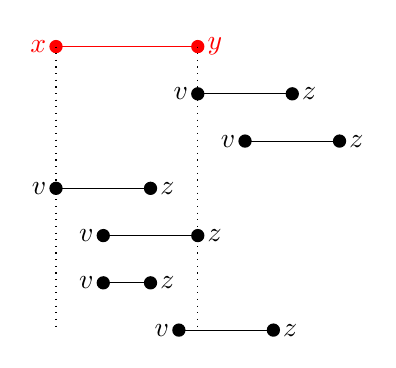
\begin{tikzpicture}[scale=1.2]
\draw[draw=none,use as bounding box](-0.3,0.2) rectangle (3.3,-3.1);
\coordinate [label=left:\textcolor{red}{$x$}] (A0) at (0,0);
\coordinate [label=right:\textcolor{red}{$y$}] (B0) at (1.5,0);
\draw[red] (A0) -- (B0);
\fill [red] (A0) circle (2pt);
\fill [red] (B0) circle (2pt);

\coordinate [label=left:$v$] (A) at (1.5,-0.5);
\coordinate [label=right:$z$] (B) at (2.5,-0.5);
\draw[black] (A) -- (B);
\fill [black] (A) circle (2pt);
\fill [black] (B) circle (2pt);

\coordinate [label=left:$v$] (A) at (2,-1);
\coordinate [label=right:$z$] (B) at (3,-1);
\draw[black] (A) -- (B);
\fill [black] (A) circle (2pt);
\fill [black] (B) circle (2pt);

\coordinate [label=left:$v$] (A) at (0,-1.5);
\coordinate [label=right:$z$] (B) at (1,-1.5);
\draw[black] (A) -- (B);
\fill [black] (A) circle (2pt);
\fill [black] (B) circle (2pt);

\coordinate [label=left:$v$] (A) at (0.5,-2);
\coordinate [label=right:$z$] (B) at (1.5,-2);
\draw[black] (A) -- (B);
\fill [black] (A) circle (2pt);
\fill [black] (B) circle (2pt);

\coordinate [label=left:$v$] (A) at (0.5,-2.5);
\coordinate [label=right:$z$] (B) at (1,-2.5);
\draw[black] (A) -- (B);
\fill [black] (A) circle (2pt);
\fill [black] (B) circle (2pt);

\coordinate [label=left:$v$] (A) at (1.3,-3);
\coordinate [label=right:$z$] (B) at (2.3,-3);
\draw[black] (A) -- (B);
\fill [black] (A) circle (2pt);
\fill [black] (B) circle (2pt);

\coordinate (A1) at (0,-3);
\coordinate (B1) at (1.5,-3);
\draw[dotted] (A0) -- (A1);
\draw[dotted] (B0) -- (B1);
\end{tikzpicture}